\documentclass[12pt]{article}
\usepackage{amsmath}
\usepackage{array}
\usepackage[thinc]{esdiff}
% \usepackage{gensymb}
\usepackage{geometry}
\usepackage{graphicx}
\usepackage{pgfplots}
\usepackage{siunitx}
\usepackage{wrapfig}

\title{Homework \#4, 4B}
\author{Donald Aingworth IV}
\date{February 12, 2025}

\pgfplotsset{width=8cm,compat=1.9}
\usepgfplotslibrary{external}
% \tikzexternalize

\renewcommand\thesubsection{\alph{subsection}}

\begin{document}

\DeclareSIUnit{\mile}{mi}
\DeclareSIUnit{\gal}{gal}
\DeclareSIUnit{\foot}{ft}
\DeclareSIUnit{\hour}{h}
\DeclareSIUnit{\rad}{rad}
\DeclareSIUnit{\unit}{u}
\DeclareSIUnit{\dyne}{dyn}

\maketitle


\section{Problem 33}
\begin{wrapfigure}{r}{0.5\textwidth}
    \vspace{-30pt}
    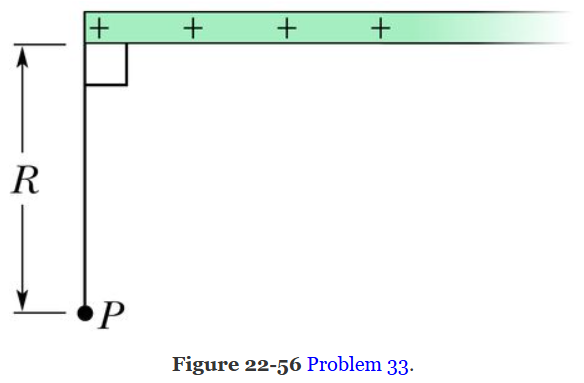
\includegraphics[width=0.5\textwidth]{picture_1.png} 
    % \label{fig:wrapfig}
\end{wrapfigure}
Fig. 22-56, a ``semi-infinite" nonconducting rod (that is, infinite in one direction only) has uniform linear charge density $\lambda$. Show that the electric field $E_p$ at point $P$ makes an angle of 45\unit{\degree} with the rod and that this result is independent of the distance $R$. (Hint: separately find the component of $E_p$ parallel to the rod and the component perpendicular to the rod.)

\subsection*{Solution}
We will be using vector formatting. We can use the formula for electric field at a point. We also find the formula for the charge density.
\begin{align*}
    \lambda &=  \frac{Q}{x} \rightarrow
    dq  =   \lambda dx\\
    \vec{E} &=  \int_{0}^{\infty} d\vec{E}
        =   \int_{0}^{\infty} \frac{k dq}{r^2} \hat{r}
        =   \int_{0}^{\infty} \frac{k \lambda}{r^2} \hat{r} dx
        =   \int_{0}^{\infty} \frac{k \lambda}{r^3} \vec{r} dx
        =   \int_{0}^{\infty} \frac{k \lambda}{(x^2 + R^2)^{3/2}} \begin{pmatrix}x\\-R\end{pmatrix} dx\\
        &=  \int_{0}^{\infty} \frac{k \lambda}{(x^2 + R^2)^{3/2}} \begin{pmatrix}x\\-R\end{pmatrix} dx
        =   k \lambda \int_{0}^{\infty} \frac{1}{(x^2 + R^2)^{3/2}} \begin{pmatrix}x\\-R\end{pmatrix} dx\\
        &=  k \lambda \int_{0}^{\infty} \frac{x}{(x^2 + R^2)^{3/2}} \begin{pmatrix}1\\0\end{pmatrix} - \frac{R}{(x^2 + R^2)^{3/2}} \begin{pmatrix}0\\1\end{pmatrix} dx\\
        &=  k \lambda \left[-\frac{1}{\sqrt{x^2 + R^2}} \begin{pmatrix}1\\0\end{pmatrix} - \frac{xR}{R^2\sqrt{x^2 + R^2}} \begin{pmatrix}0\\1\end{pmatrix}\right]_{x=0}^{\infty}\\
        &=  -k\lambda \left[\left(\frac{1}{\sqrt{\infty^2 + R^2}} - \frac{1}{\sqrt{0^2 + R^2}}\right) \begin{pmatrix}1\\0\end{pmatrix} + \left(\frac{\infty}{R\sqrt{\infty^2 + R^2}} - \frac{0}{R\sqrt{0^2 + R^2}}\right) \begin{pmatrix}0\\1\end{pmatrix}\right]\\
        &=  -k\lambda \left[-\frac{1}{R} \begin{pmatrix}1\\0\end{pmatrix} + \right]
\end{align*}

From here on out, we can focus only on the x-component.
\begin{align*}
    E_x &=  -k\lambda \frac{-R^2}{y^2\sqrt{R^2 + y^2} + y(R^2 + y^2)}
        =   \frac{k\lambda R^2}{y} \cdot \frac{1}{y\sqrt{R^2 + y^2} + R^2 + y^2}
\end{align*}

\pagebreak
\section{Problem 50}
At some instant the velocity components of an electron moving between two charged parallel plates are $v_x = 1.5 \times 10^5 \unit{\meter/\second}$ and $v_y = 3.0 \times 10^3 \unit{\meter/\second}$. Suppose the electric field between the plates is uniform and given by $\vec{E} = (120 \unit{\newton/\coulomb})\hat{j}$. In unit-vector notation, what are (a) the electron's acceleration in that field and (b) the electron's velocity when its x coordinate has changed by 2.0 cm?

\subsection{Solution: Acceleration in the field}
The acceleration can be found with the formula from Newton's second law \(\vec{a} = \frac{\vec{F}}{m}\).
With the relationship between the force and the electric field \(\vec{F} = q\vec{E}\), we can get the updated formula \(\vec{a} = \frac{q\vec{E}}{m}\). 
We can plug values into that relationship to find the solution, keeping in mind that the mass of an electron is $9.109 \times 10^{-31} \unit{\kilo\gram}$ and the charge of an electron is $-1.602 \times 10^{-19} \unit{\coulomb}$.
\begin{align*}
    \vec{a} &=  \frac{q\vec{E}}{m} = \frac{(-1.602 \times 10^{-19} \unit{\coulomb})(120 \unit{\newton/\coulomb})\hat{j}}{9.109 \times 10^{-31}\ \unit{\kilo\gram}}\\
        &=  -\frac{1.602 * 1.20}{9.109} \times 10^{14}\hat{j}\ \unit{\meter/\second^2}\\
        &=  -\frac{1.9224}{9.109} \times 10^{14}\hat{j}\ \unit{\meter/\second^2}
        =   \boxed{-2.110 \times 10^{13} \hat{j}\ \unit{\meter/\second^2}}
\end{align*}

\subsection{Solution: Velocity after going 2.0 cm}
We first calculate the time that the electron would take to travel 2.0 cm (or 0.02 m) in the horizontal direction. Since there is no horizonatal acceleration, we just need to use a simple formula.
\begin{equation*}
    x_f =   x_i + v_x t\rightarrow\\
    t   =   \frac{\Delta x}{v_x}
        =   \frac{2 \times 10^{-2}}{1.5 \times 10^5}
        =   \frac{4}{3} \times 10^{-7} \unit{\second}
\end{equation*}

Next, we calculate the velocity after this time, using the first kinematic equation. 
\begin{align*}
    v_f &=  v_i + at
        =   3.0 \times 10^3 \unit{\meter/\second} + (-2.110 \times 10^{13} \unit{\meter/\second^2})(\frac{4}{3} \times 10^{-7} \unit{\second})\\
        &=  3.0 \times 10^3 \unit{\meter/\second} - 2.81 \times 10^6 \unit{\meter/\second}
        =   -2.81 \times 10^6 \unit{\meter/\second}\\
    v   &=  \boxed{\left(\begin{matrix} 1.5 \times 10^5 \\ -2.81 \times 10^6 \end{matrix}\right) \unit{\meter/\second}}
\end{align*}

\pagebreak
\section{Problem 55}
A uniform electric field exists in a region between two oppositely charged plates. An electron is released from rest at the surface of the negatively charged plate and strikes the surface of the opposite plate, 2.0 cm away, in a time $1.5 \times 10^{-8} \unit{\second}$. (a) What is the speed of the electron as it strikes the second plate? (b) What is the magnitude of the electric field $\vec{E}$?

\subsection{Solution: Speed of the electron when it strikes the other plate}
We use the kinematic equations.
\begin{gather*}
    \frac{\Delta r}{t} = \frac{\Delta v}{2}
\end{gather*}
Since the initial position and velocity are both zero, we can replace $\Delta r$ with $r_f$ and $\Delta v$ with $v_f$.
\begin{gather*}
    \frac{r_f}{t}   =   \frac{v_f}{2}\\
    v_f =   \frac{2r_f}{t}
        =   \frac{4 \times 10^{-2}}{1.5 \times 10^{-8}}
        =   \boxed{\frac{8}{3} \times 10^6 \unit{\meter/\second}}
\end{gather*}

\subsection{Solution: Electric field magnitude}
We start with the electric field and use formulae to get to the values we do know, assuming a constant acceleration.
\begin{gather*}
    E = \frac{F}{q}\\
    E = \frac{ma}{q}\\
    E = \frac{mv}{qt}
\end{gather*}
From that, we then plug values in to get the magnitude of the electric field.
\begin{align*}
    E   &=  \frac{qmv}{t}
        =   \frac{(9.109 \times 10^{-31})(\frac{8}{3} \times 10^6)}{(1.602 \times 10^{-19})(1.5 \times 10^{-8})}\\
        &=  \frac{72.872 \times 10^{33}}{7.209 \times 10^{31}}
        =   \boxed{1.011 \times 10^3 \unit{\newton/\coulomb}}
\end{align*}

\pagebreak
\section{Problem 59}
How much work is required to turn an electric dipole 180\unit{\degree} in a uniform electric field of magnitude E = 46.0 N/C if the dipole moment has a magnitude of $p = 3.02 \times 10^{-25} \unit{\coulomb\cdot\meter}$ and the initial angle is 64\unit{\degree}?

\subsection*{Solution}
\begin{align*}
    W   &=  -\Delta U
        =   U_i - U_f
        =   (-Ep\cos(\theta_i)) - (-Ep\cos(\theta_f))\\
        &=  Ep\cos(\theta_f) - Ep\cos(\theta_i)
        =   Ep(\cos(\theta_f) - \cos(\theta_i))\\
        &=  (46.0)(3.02 \times 10^{-25})(\cos(244 \unit{\degree}) - \cos(64 \unit{\degree})) \unit{\newton\cdot\meter}\\
        &=  (138.92 \times 10^{-25})(-0.8767) \unit{\joule}
        =   \boxed{-1.21797 \times 10^{-23} \unit{\joule}}
\end{align*}

\pagebreak
\section{Problem 60}
\begin{wrapfigure}{r}{0.25\textwidth}
    \vspace{-30pt}
    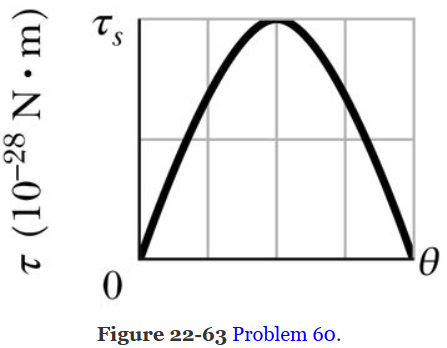
\includegraphics[width=0.25\textwidth]{picture_5.png} 
    % \label{fig:wrapfig}
\end{wrapfigure}
A certain electric dipole is placed in a uniform electric field E of magnitude 40 N/C. Figure 22-63 gives the magnitude $\tau$ of the torque on the dipole versus the angle $\theta$ between field E and the dipole moment p. The vertical axis scale is set by $\tau_s = 100 \times 10^{-28} \unit{\newton\cdot\meter}$. What is the magnitude of p?

\subsection*{Solution}
Since we're working with magnitudes, we can use magnitude-based formulas, notably \(\tau = pE\sin(\theta)\). 
Since the first peak of the sine function is at $\theta = \frac{\pi}{2}$, the value of $\sin(\theta)$ would be 1 at the peak. 
We can then use it for the aforementianed magnitude-based formula.
\begin{gather*}
    \tau_s  =   pE\sin(\theta)\\
    p   =   \frac{\tau_s}{E\sin(\theta)}\\
    p   =   \frac{100 \times 10^{-28}}{40}
        =   \boxed{2.5 \times 10^{-28} \unit{\coulomb*\meter}}
\end{gather*}

\pagebreak
\section{Problem 76}
\begin{wrapfigure}{r}{0.15\textwidth}
    \vspace{-30pt}
    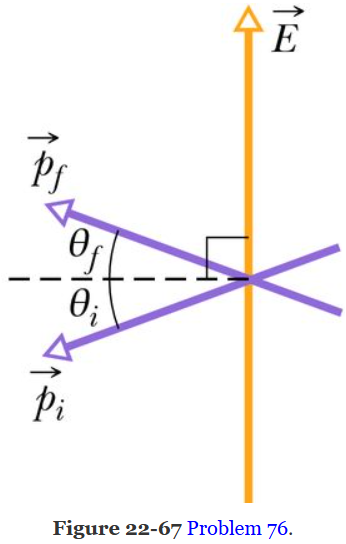
\includegraphics[width=0.15\textwidth]{picture_6.png} 
    % \label{fig:wrapfig}
\end{wrapfigure}
In Fig. 22-67, an electric dipole swings from an initial orientation $i (\theta_i = 20.0\unit{\degree})$ to a final orientation $f (\theta_f= 20.0\unit{\degree})$ in a uniform external electric field E. The electric dipole moment is $1.60 \times 10^{-37} \unit{\coulomb\cdot\meter}$; the field magnitude is $3.00 \times 10^6 \unit{\newton/\coulomb}$. What is the change in the dipole's potential energy?

\subsection*{Solution}
The initial orientation makes an angle of 90\unit{\degree} + 20\unit{\degree} = 110\unit{\degree} with the electric field.
The final orientation makes an angle of 90\unit{\degree} - 20\unit{\degree} = 70\unit{\degree} with the electric field.
We can then use the formula for the change in the dipole's potential energy to find the solution.
\begin{align*}
    W   &=  -\Delta U
        =   U_i - U_f
        =   (-Ep\cos(\theta_i)) - (-Ep\cos(\theta_f))\\
        &=  Ep\cos(\theta_f) - Ep\cos(\theta_i)
        =   Ep(\cos(\theta_f) - \cos(\theta_i))\\
        &=  (3.0 \times 10^6)(1.60 \times 10^{-37})(\cos(110\unit{\degree}) - \cos(70\unit{\degree}))\\
        &=  \left(4.8 \times 10^{-31}\right)\left(-2\sin\left(\frac{\pi}{9}\right)\right)
        =   \boxed{-3.283 \times 10^{-31} \unit{\joule}}
\end{align*}
\end{document}